\documentclass[12pt]{article}
            \usepackage{sbc-template}
            \makeatletter
            \renewcommand{\inst}[1]{}
            \makeatother
            \usepackage{graphicx,url}
            \usepackage[utf8]{inputenc}
            \usepackage[T1]{fontenc}
            \usepackage[brazil]{babel}
            \usepackage{longtable,booktabs,array,tabularx}
            \usepackage{amsmath,amssymb}
            \usepackage{fvextra}
            \newcolumntype{Y}{>{\raggedright\arraybackslash}X}
            \newcolumntype{C}{>{\centering\arraybackslash}X}
            \setlength{\LTleft}{0pt}
            \setlength{\LTright}{0pt}
            \RecustomVerbatimEnvironment{verbatim}{Verbatim}{%
              breaklines=true,
              breakanywhere=true,
              breaksymbolleft={},
              fontsize=\small
            }
            \providecommand{\tightlist}{%%
              \setlength{\itemsep}{0pt}\setlength{\parskip}{0pt}}
            \providecommand{\pandocbounded}[1]{#1}
            \usepackage{fancyhdr}
            \pagestyle{fancy}
            \fancyhf{}
            \fancyfoot[R]{\thepage}
            \fancyfoot[L]{SANTOS, Anderson F. P. dos — RC físico e ponte para QRC}
            \renewcommand{\headrulewidth}{0pt}
            \renewcommand{\footrulewidth}{0.4pt}
            \sloppy
            \title{RC físico e ponte para QRC}
            \author{Anderson Fernandes Pereira dos Santos}
            \address{Instituto Militar de Engenharia (IME), Rio de Janeiro, Brazil \\
Venturus Innovation Center, Campinas, Brazil \\
\texttt{anderson@ime.eb.br} | \texttt{anderson.santos@venturus.org.br}}
            \begin{document}

            \maketitle

            \begin{resumo}
            Este artigo constroi a ponte entre o RC clássico estudado até aqui e o QRC usado no estudo final. O objetivo é mostrar que QRC não nasce como um tema separado do restante da obra, mas como uma extensão natural da ideia de reservatório: manter a separacao entre dinâmica rica e readout simples, trocando o meio clássico por um meio quântico. O texto apresenta o paralelo formal entre RC e QRC, mapeia essa ponte para a implementação em Qiskit, discute a estrategia de tuning usada no projeto e introduz a função objetivo que equilibra desempenho e complexidade (\texttt{qubits}, \texttt{window}). Ao final, o leitor sabe por que duas configurações candidatas emergiram do tuning: \texttt{14x7} como melhor ponto multi-métrica e \texttt{8x5} como melhor compromisso segundo a função objetivo escalar.
            \end{resumo}

            \section{O que o leitor vai aprender}\label{1-o-que-o-leitor-vai-aprender}

Ao final deste artigo, você será capaz de:

\begin{enumerate}
\def\labelenumi{\arabic{enumi}.}
\tightlist
\item
  enxergar RC e QRC dentro do mesmo paradigma;
\item
  entender como entradas clássicas sao codificadas em circuitos quânticos;
\item
  ler a implementação do QRC em \texttt{code/qrc/model.py};
\item
  interpretar o tuning de \texttt{n\_qubits} e \texttt{window};
\item
  justificar tecnicamente por que \texttt{14x7} e \texttt{8x5} foram preservados para o artigo final.
\end{enumerate}

\section{RC como paradigma geral}\label{2-rc-como-paradigma-geral}

No RC clássico, a ideia e:

\[
u_t \longrightarrow x_t \longrightarrow \phi_t \longrightarrow \hat{y}_t.
\]

Em outras palavras:

\begin{itemize}
\tightlist
\item
  a entrada \(u_t\) perturba um sistema dinamico;
\item
  o sistema responde com um estado \(x_t\);
\item
  o readout linear aprende a ler esse estado.
\end{itemize}

O QRC preserva exatamente essa lógica. O que muda e o meio em que a dinâmica interna acontece.

\section{O salto para o quântico}\label{3-o-salto-para-o-quuxe2ntico}

No projeto, o reservatório quântico usa circuitos de reuploading implementados com Qiskit. Para cada qubit \(q\) e para cada passo de entrada, a codificacao usa angulos do tipo

\[
\theta^{(q,t)}_x = s \, w_{x,q}^\top u_t + b_q,
\qquad
\theta^{(q,t)}_y = s \, w_{y,q}^\top u_t,
\]

em que:

\begin{itemize}
\tightlist
\item
  \(u_t \in \mathbb{R}^4\) é o vetor clássico reduzido;
\item
  \(s\) e \texttt{input\_scale};
\item
  \(w_{x,q}\) e \(w_{y,q}\) sao pesos aleatórios por qubit.
\end{itemize}

O circuito elementar do projeto aplica:

\begin{enumerate}
\def\labelenumi{\arabic{enumi}.}
\tightlist
\item
  \texttt{RX} e \texttt{RY} em cada qubit;
\item
  um anel de emaranhamento \texttt{CZ};
\item
  rotações \texttt{RZ} apos cada acoplamento.
\end{enumerate}

\section{Paralelo direto entre RC e QRC}\label{4-paralelo-direto-entre-rc-e-qrc}

O paralelo conceitual entre os dois modelos pode ser escrito assim:

\begin{longtable}[]{@{}ll@{}}
\toprule\noalign{}
RC clássico & QRC do projeto \\
\midrule\noalign{}
\endhead
\bottomrule\noalign{}
\endlastfoot
estado vetorial \(x_t\) & estado quântico \(\lvert\psi_t\rangle\) \\
matriz recorrente \(W_{res}\) & circuito com \texttt{RX}, \texttt{RY}, \texttt{CZ}, \texttt{RZ} \\
features \([1; u_t; x_t]\) & features \([1; u_t; z_t]\) \\
readout linear & readout linear \\
\end{longtable}

No QRC, as features observadas sao expectativas de operadores:

\[
z_t^{(j)} = \langle \psi_t | O_j | \psi_t \rangle.
\]

No projeto, cada configuração com \(n_{\text{qubits}} = q\) gera \(3q\) observáveis:

\begin{itemize}
\tightlist
\item
  \(q\) observáveis \(Z\);
\item
  \(q\) observáveis \(X\);
\item
  \(q\) observáveis \(ZZ\) entre vizinhos.
\end{itemize}

Isso significa que:

\begin{itemize}
\tightlist
\item
  \texttt{8x5} usa \(24\) observáveis e um vetor final com \(1 + 4 + 24 = 29\) features;
\item
  \texttt{14x7} usa \(42\) observáveis e um vetor final com \(1 + 4 + 42 = 47\) features.
\end{itemize}

\section{Como o projeto implementa essa ponte em Qiskit}\label{5-como-o-projeto-implementa-essa-ponte-em-qiskit}

O passo central de codificacao esta em \texttt{\_step\_circuit()}:

\begin{verbatim}
for q in range(self.config.n_qubits):
    angle_x = self.config.input_scale * float(self.rx_weights[q] @ input_vector) + self.bias[q]
    angle_y = self.config.input_scale * float(self.ry_weights[q] @ input_vector)
    circuit.rx(angle_x, q)
    circuit.ry(angle_y, q)
\end{verbatim}

O emaranhamento em anel aparece logo em seguida:

\begin{verbatim}
for q in range(self.config.n_qubits - 1):
    circuit.cz(q, q + 1)
    circuit.rz(self.entangling_angles[q], q + 1)
circuit.cz(self.config.n_qubits - 1, 0)
circuit.rz(self.entangling_angles[-1], 0)
\end{verbatim}

E as features sao extraidas via \texttt{Statevector.expectation\_value()}:

\begin{verbatim}
state = Statevector.from_instruction(circuit)
features = [float(np.real(state.expectation_value(obs))) for obs in self.observables]
\end{verbatim}

Essa implementação e importante pedagogicamente porque mostra que o QRC do projeto não é uma caixa preta: ele e um pipeline legivel, curto e comparavel ao RC clássico.

\section{Tuning de qubits e window}\label{6-tuning-de-qubits-e-window}

O tuning focalizado do projeto produziu a seguinte faixa superior de configurações:

\begin{table}[htbp]
\centering
\footnotesize
\setlength{\tabcolsep}{3pt}
\begin{tabularx}{\linewidth}{@{}llCCCCC@{}}
\toprule
Qubits & Window & \shortstack{MAE\\medio} & \shortstack{RMSE\\medio} & \shortstack{WAPE\\medio} & \shortstack{sMAPE\\medio} & \shortstack{Rank\\medio} \\
\midrule
14 & 7 & 436.819 & 522.161 & 0.2017 & 0.2265 & 1.25 \\
12 & 9 & 445.061 & 524.709 & 0.2055 & 0.2306 & 2.25 \\
5 & 7 & 445.920 & 530.752 & 0.2059 & 0.2313 & 3.50 \\
8 & 5 & 447.947 & 520.913 & 0.2068 & 0.2313 & 3.50 \\
12 & 3 & 447.168 & 540.572 & 0.2065 & 0.2319 & 4.50 \\
\bottomrule
\end{tabularx}
\end{table}

\begin{figure}[htbp]
\centering
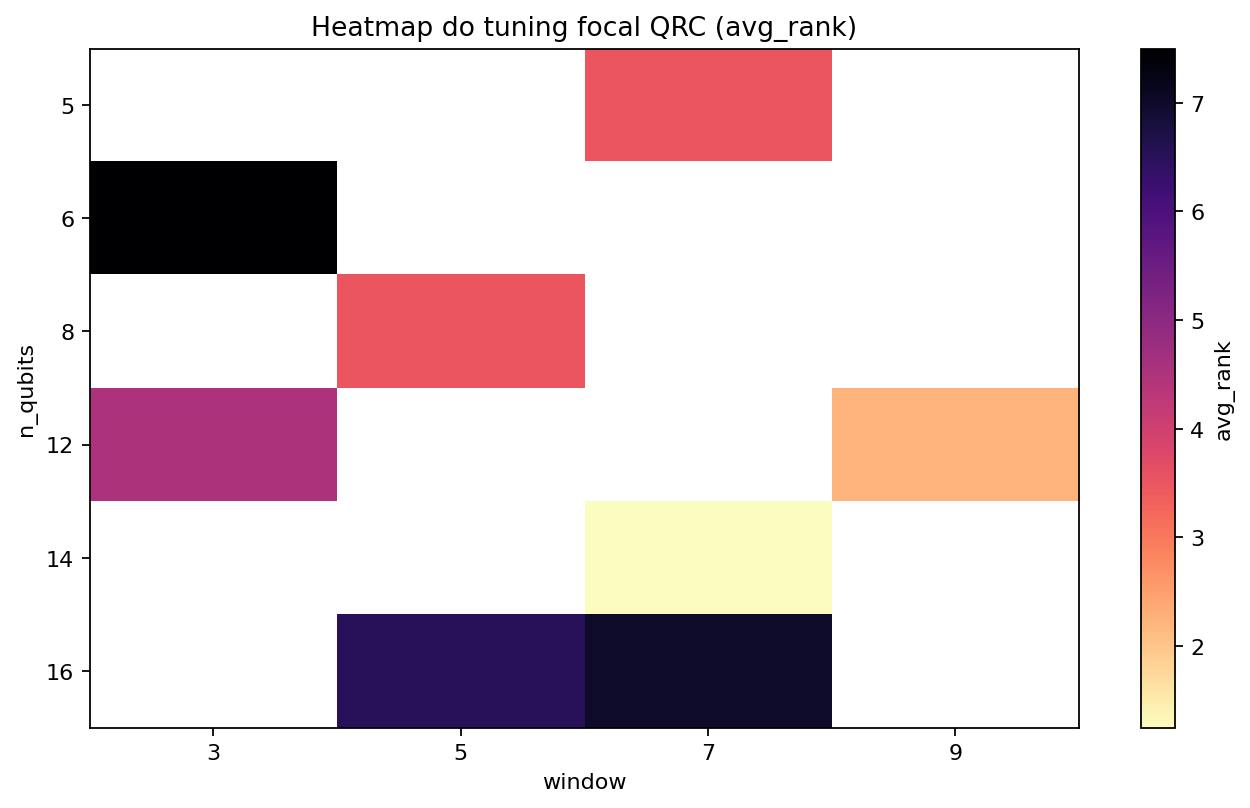
\includegraphics[width=\linewidth,keepaspectratio]{computational_results_20260402_222902/qrc_tuning_heatmap.png}
\caption{Mapa de calor do tuning de qubits e window para o QRC.}
\end{figure}

A tabela mostra uma licao decisiva: aumentar \texttt{n\_qubits} e \texttt{window} não melhora automaticamente o desempenho. O melhor ponto robusto ficou em \texttt{14x7}, enquanto \texttt{16x5} e \texttt{16x7} pioraram o rank médio.

\section{Uma função objetivo para escolher configurações comparaveis}\label{7-uma-funuxe7uxe3o-objetivo-para-escolher-configurauxe7uxf5es-comparaveis}

O projeto não ficou preso a um único critério. Além do rank médio multi-métrica, foi proposta uma função objetivo escalar

\[
J(q, w) = G(q, w) \cdot C(q, w),
\]

com

\[
G(q, w) = \exp\left(\sum_k \omega_k \log\frac{m_k(q, w)}{r_k}\right),
\]

e

\[
C(q, w) = 1 + \lambda \, \frac{\mathrm{norm}(q) + \mathrm{norm}(w)}{2}.
\]

Aqui:

\begin{itemize}
\tightlist
\item
  \(m_k(q, w)\) sao as métricas do QRC;
\item
  \(r_k\) sao as métricas da melhor referencia não-QRC;
\item
  \(\omega_k\) sao pesos por métrica;
\item
  \(\lambda = 0.05\) penaliza complexidade adicional.
\end{itemize}

Os pesos usados foram:

\begin{itemize}
\tightlist
\item
  \texttt{MAE\ =\ 0.3}
\item
  \texttt{RMSE\ =\ 0.3}
\item
  \texttt{WAPE\ =\ 0.2}
\item
  \texttt{sMAPE\ =\ 0.2}
\end{itemize}

O resumo da selecao ficou assim:

\begin{longtable}[]{@{}lll@{}}
\toprule\noalign{}
Critério & Melhor configuração & Valor \\
\midrule\noalign{}
\endhead
\bottomrule\noalign{}
\endlastfoot
Melhor rank médio multi-métrica & 14x7 & 1.25 \\
Melhor função objetivo escalar & 8x5 & 2.0030 \\
\end{longtable}

O critério multi-métrica favorece \texttt{14x7}. A função objetivo penalizada favorece \texttt{8x5}.

\section{O que se ganha e o que se perde na ponte para QRC}\label{8-o-que-se-ganha-e-o-que-se-perde-na-ponte-para-qrc}

\subsection{O que se ganha}\label{81-o-que-se-ganha}

\begin{itemize}
\tightlist
\item
  uma nova classe de dinâmica para representar séries temporais;
\item
  uma formulação muito natural para discutir observáveis e mistura de estados;
\item
  uma extensão conceitual elegante do paradigma de reservatório.
\end{itemize}

\subsection{O que se perde}\label{82-o-que-se-perde}

\begin{itemize}
\tightlist
\item
  simplicidade operacional em relação ao RC clássico;
\item
  custo computacional, especialmente quando \texttt{qubits} e \texttt{window} crescem;
\item
  interpretabilidade imediata do estado interno.
\end{itemize}

\section{Por que o benchmark anterior precisa ser herdado}\label{9-por-que-o-benchmark-anterior-precisa-ser-herdado}

O QRC só faz sentido pedagógico neste projeto porque herda o benchmark do artigo 5. Sem esse benchmark, seria fácil tratar o QRC como curiosidade isolada. Com ele, o leitor entende exatamente contra o que o QRC precisa ser comparado:

\begin{itemize}
\tightlist
\item
  \texttt{ETS}
\item
  \texttt{XGBoost}
\item
  \texttt{Prophet}
\item
  \texttt{Seasonal\ Naive}
\item
  \texttt{RC}
\item
  \texttt{LSTM}
\end{itemize}

Essa heranca metodológica e o que impede a fase quântica de perder contato com o problema de negócio.

\section{Conclusão}\label{10-conclusuxe3o}

A ponte entre RC clássico e QRC esta pronta. O leitor agora tem um mapa formal, implementacional e experimental do salto para o quântico. O artigo final vai aproveitar exatamente essa ponte para executar e interpretar o QRC no recorte adotado no Favorita, comparando \texttt{14x7}, \texttt{8x5} e os melhores modelos clássicos.

\section*{Entregaveis associados no repositorio}\label{entregaveis-associados-no-repositorio}

\begin{itemize}
\tightlist
\item
  implementação do QRC: \texttt{code/qrc/model.py}
\item
  função objetivo: \texttt{code/qrc/objective.py}
\item
  documentacao da função objetivo: \texttt{code/qrc/OBJECTIVE.md}
\item
  artefatos deste artigo: \texttt{computational\_results\_20260402\_222902/}
\end{itemize}

\section{Referências}\label{referencias}

\begin{thebibliography}{9}

\bibitem{jaeger2001}
JAEGER, H. \textbf{The ``echo state'' approach to analysing and training recurrent neural networks}. Bonn: German National Research Center for Information Technology (GMD), 2001.

\bibitem{lukosevicius2009}
LUKOSEVICIUS, M.; JAEGER, H. \textbf{Reservoir computing approaches to recurrent neural network training}. \emph{Computer Science Review}, v. 3, n. 3, p. 127--149, 2009.

\bibitem{lukosevicius2012}
LUKOSEVICIUS, M. \textbf{A practical guide to applying echo state networks}. In: MONTAVON, G.; ORR, G. B.; MÜLLER, K.-R. (org.). \emph{Neural Networks: Tricks of the Trade}. 2. ed. Berlin: Springer, 2012. p. 659--686.

\bibitem{fujii2017}
FUJII, K.; NAKAJIMA, K. \textbf{Harnessing disordered-ensemble quantum dynamics for machine learning}. \emph{Physical Review Applied}, v. 8, n. 2, 024030, 2017.

\end{thebibliography}

            \end{document}
